\chapter{Botnets}
As Botnets são redes formadas por máquinas infectadas com \textit{malware}, permitindo que o atacante (\textit{botmaster}) realize diversas atividades criminais remotamente, como roubo de informações, ataques de negação de serviço, envio de SPAM, etc. \citep{silva2013botnets}.

Com o crescimento e diversificação do uso da Internet, o meio cibernético se tornou mais relevante e mais atraente para a realização de ataques maliciosos. Isso motivou o crescimento do número de botnets existentes e aumentou o potencial de contaminação das mesmas, além disso, para evitar os mecanismos de detecção existentes, elas se tornaram cada vez mais sofisticadas.

Para que o detector se torne mais robusto, é preciso compreender o funcionamento das botnets e seus objetivos. Esse conhecimento é necessário para entender as configurações existentes nas botnets atuais, além de compreender como essas configurações podem evoluir. De posse desse conhecimento, espera-se que seja possível identificar características relevantes e intrínsecas ao funcionamento das botnets, mesmo quando o \textit{botmaster} estiver tentando evitar os mecanismos de detecção.

\section{Elementos das Botnets}
As botnets apresentam alguns elementos estruturais tipicamente envolvidos, que estão presentes independente do protocolo ou arquitetura utilizada. A Figura \ref{fig:typical_elements} mostra a estrutura desses elementos e como eles se relacionam em uma botnet. Segue uma descrição para cada componente:
\begin{itemize}  
\item Bots: São \textit{malwares} instalados nos computadores das vítimas que podem realizar as ações maliciosas que o \textit{botmaster} envia através do canal de comando e controle (C\&C). Geralmente, o \textit{malware} é inicializado quando o hospedeiro inicializa a máquina, porém isso pode ser configurado pelo \textit{botmaster} para dificultar a detecção da atividade maliciosa.
\item Hospedeiros: São as máquinas em que o bot foi instalado, ou seja, infectadas \citep{puri2003bots}.
\item \textit{Botmaster}: é o indivíduo que configura o bot, dissemina e controla a botnet.
\item Canal de Comando e Controle (C\&C): é o meio que o \textit{botmaster} tem para se comunicar com a sua botnet. É a parte chave do funcionamento, pois é necessário para o envio dos comandos de atividade maliciosa aos hospedeiros. Dessa forma, grande parte das características da botnet, como robustez, facilidade de detecção/desativação, estabilidade, etc., são definidas pela forma que a infraestrutura de C\&C está organizada.
\end{itemize}

\begin{figure}
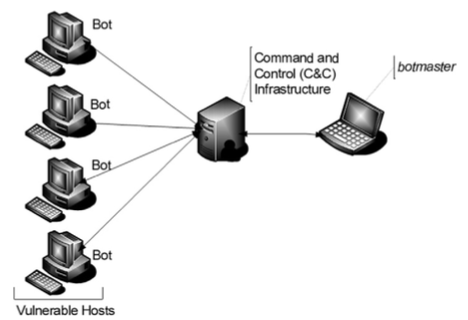
\includegraphics[width=\textwidth]{typical_elements}
\caption[Elementos das botnets]{Elementos das botnets \citep{silva2013botnets}} \label{fig:typical_elements}
\end{figure}

\section{Ameaças e Formas de Defesa}
O crescimento do número de máquinas conectadas constantemente a enlaces de alta velocidade e rodando sistemas com vulnerabilidades consideráveis, criou um ambiente favorável à formação de botnets. Além disso, muitas vezes o bot é transparente ao responsável pela máquina infectada, ou seja, não atrapalha o funcionamento da máquina, fazendo com que a vítima não perceba a infecção e tente combatê-la. Esses fatores, aliados ao enorme potencial de causar danos, fazem com que as botnets sejam um dos maiores desafios de pesquisa em segurança no espaço cibernético atual \citep{soltani2014survey}.

Existem características que tornam o \textit{host} mais interessante ao \textit{botmaster} como: altas taxas de transmissão, baixos níveis de segurança e monitoração, alta disponibilidade e localização distante (dificultando que as agências reguladoras detectem as atividades, já que os bots estarão espalhados por diversas nações). Esses fatores ajudam o bot a passar desapercebido e a contribuir com maior capacidade de banda ao \textit{botmaster}, facilitando ataques como os de negação de serviço.

Existem duas formas para combater um ataque realizado por botnets: reativamente ou preventivamente. A forma reativa é a mais comum e envolve detectar a existência da atividade maliciosa e reagir ao ataque tentando reduzir o tráfego malicioso para níveis aceitáveis. Uma desvantagem é que o ataque já vai ter sido inicializado quando for detectado, ou seja, já vai haver causado danos antes de ser solucionado. A forma preventiva busca evitar que a botnet possa realizar alguma atividade maliciosa, porém essa atividade não é simples, já que o atacante pode aprimorar seus bots, tornando-os mais sofisticados, exigindo grandes investimentos para manter os recursos de segurança atualizados.

O mecanismo que estamos desenvolvendo é da forma preventiva, já que o algoritmo busca encontrar padrões e identificar possíveis máquinas infectadas por botnets. Tudo isso na fase em que o \textit{botmaster} ainda está infectando máquinas com o bot para a botnet. Ou seja, buscamos detectar as máquinas infectadas antes do ataque, como um ataque de negação de serviço, em si ser efetivado. Uma característica desejável para um detector é a detecção em tempo real, com o objetivo de minimizar os danos causados e o tempo de reação do \textit{botmaster}. Porém, obter essa característica é um desafio, devido ao grande número de dados que devem ser tratados e analisados. Dessa forma, nosso projeto não fará detecção em tempo real, mas tentará se aproximar disso, utilizando a detecção dos dados coletados ao longo de um dia para detectar bots que atuaram nas últimas 24 horas.

\section{Ciclo de Vida das Botnets}
Na maioria dos casos, existe um ciclo com fases bem definidas de como uma botnet é criada e mantida, a Figura \ref{fig:botnets_lifecycle} mostra essas fases para cada novo hospedeiro que é contaminado.

\begin{figure}
\tikzstyle{block} = [rectangle, draw, text width=9em, text centered, rounded corners, minimum height=4em]
\tikzstyle{line} = [draw, -latex']
\centering
\begin{tikzpicture}[node distance = 4.5cm, auto]
    % Place nodes
    \node [block] (init) {Infecção Inicial};
    \node [block, below of=init] (second) {Injeção Secundária};
    \node [block, right of=init] (connection) {Conexão};
    \node [block, below of=connection] (malicious) {Atividades Maliciosas};
    \node [block, right of=malicious] (update) {Manutenção e Atualização};
    % Draw edges
    \path [line] (init) -- (second);
    \path [line] (second) -- (connection);
    \path [line] (connection) |- +(4,2) |- (connection.east); 
    \path [line] (connection) -- (malicious);
    \path [line] (malicious) -- (update);
    \path [line] (update) -- (connection);

\end{tikzpicture}
\caption[Ciclo de Vida das Botnets]{Ciclo de Vida das Botnets} \label{fig:botnets_lifecycle}
\end{figure}

Na primeira fase, chamada de injeção inicial, o atacante procura vulnerabilidades na máquina do futuro hospedeiro para explorá-las e infectá-lo com o \textit{malware}, tornando-se um bot em potencial, isso pode ocorrer, por exemplo, através de um \textit{download} indesejado ou através de um anexo em um e-mail. Após a infecção ser bem sucedida, ocorre a injeção secundária: o host infectado, através do \textit{malware} inicial instalado, busca em uma rede os reais binários do \textit{malware} do bot, os quais após baixados e executados concluirão a infecção e transformam o host em um bot real.\citep{feily2009survey}

Durante a fase de conexão, o bot estabelece conexão com o canal de C\&C. Isso se repete sempre que o host é reiniciado, podendo ser considerada uma fase vulnerável já que é uma fase essencial, além de geralmente seguir um padrão. Após a efetivação da conexão, o bot se torna ativo na botnet, e passa a realizar os comandos enviados pelo \textit{botmaster} através do canal de C\&C, efetivando as atividades maliciosas solicitadas. A última fase é a de manutenção e atualização, e tem por objetivo manter a botnet ativa e atualizada, já que se o \textit{botmaster} deseja que os bots possam evitar novas técnicas de detecção, adicionar novas funcionalidades ou até mesmo alterar o servidor de C\&C, os binários do programa bot devem ser modificados.

\section{Arquitetura das Botnets}
Existem 4 tipos de arquiteturas para as botnets: centralizada, descentralizada, híbrida e aleatória. 

Na arquitetura centralizada, mostrada na Figura \ref{fig:centralized_architecture} todos os bots se comunicam com um número pequeno de servidores de C\&C. Embora ela ofereça vantagens ao \textit{botmaster}, como baixa latência e facilidade de manutenção, ela também torna a botnet bastante vulnerável, permitindo que a botnet seja desligada após a identificação dos poucos pontos centrais de C\&C. Esta arquitetura é muito utilizada por botnets que utilizam o protocolo IRC (\textit{Internet Relay Chat}) para comunicação. Todavia, o tráfego desse protocolo é incomum e raramente utilizado, especialmente em ambientes corporativos, por esse motivo, o tráfego desse tipo de protocolo costuma ser bloqueado, inutilizando a botnet. Devido a isso, o uso do protocolo HTTP (\textit{HyperText Transfer Protocol}) se popularizou já que ele é amplamente utilizado, disfarçando as comunicações das botnets.

\begin{figure}
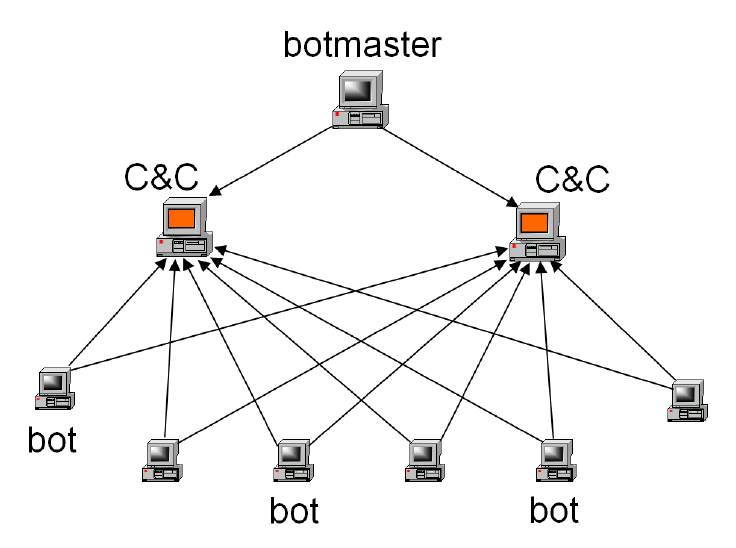
\includegraphics[width=\textwidth]{centralized}
\caption[Arquitetura Centralizada]{Arquitetura Centralizada\citep{wang2010advanced}} \label{fig:centralized_architecture}
\end{figure}

A fragilidade da arquitetura centralizada, motivou o desenvolvimento da arquitetura descentralizada, na qual uma variedade de protocolos P2P (\textit{Peer-to-peer}) é utilizada. A flexibilidade e robustez dessa arquitetura, permite que mesmo que muitos bots sejam desativados a botnet possa continuar funcionando, já que não existem pontos centralizados de C\&C. 

As arquiteturas híbridas apresentam características de ambas as arquiteturas centralizadas e descentralizadas, como mostrado na Figura \ref{fig:hybrid_architecture}, na qual os bots são classificados em dois grupos: clientes e serventes. Os serventes exercem os papéis tanto de clientes quanto servidores, possuindo endereço de IP estático e público para serem acessíveis globalmente, sendo utilizados para repassar os comandos enviados pelo \textit{botmaster}. Os demais bots, são denominados clientes pois não aceitam comunicações de entrada, dessa forma e podem apresentar IP dinâmico, privado ou protegidos por \textit{firewall} para não serem roteados facilmente. 

Por fim, a arquitetura aleatória é um modelo, até agora, apenas teórico. No qual o bot não se comunica ativamente com o \textit{botmaster} ou com outros bot. Dessa forma, para realizar um ataque, o \textit{botmaster} precisa vasculhar a rede em busca de um bot para enviar o comando e realizar as atividades maliciosas.

\begin{figure}
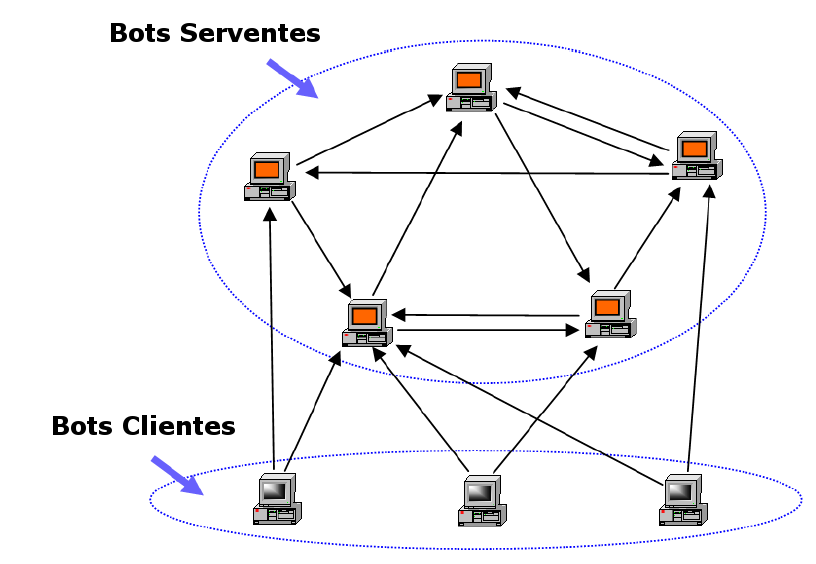
\includegraphics[width=\textwidth]{hybrid}
\caption[Arquitetura Híbrida]{Arquitetura Híbrida\citep{wang2010advanced}} \label{fig:hybrid_architecture}
\end{figure}

\section{Detecção de Botnets}

Existem duas categorias de técnicas para detecção de botnets: \textit{honeynets} e sistemas de detecção de intrusos (IDS). 

As \textit{honeynets} consistem na criação de redes que apresentam vulnerabilidades com a intenção de que elas sejam comprometidas com \textit{malwares}. Isso permite que informações sobre a botnet sejam captadas e estudadas. Por isso elas são consideradas mais efetivas para compreender as características de uma botnet do que para realizar a detecção de botnets.

A detecção por IDS, pode ser classificada entre duas técnicas: a baseada em assinaturas e a baseada em anomalias. A técnica baseada em assinaturas, consiste em extrair padrões da rede e comparar com um banco de dados onde se encontram os padrões que já foram vistos em botnets, ou seja, ela não permite que novas botnets sejam identificadas e envolve a posse de um banco de dados enorme com o maior número de informações existentes sobre as botnets previamente detectadas. Dessa forma, a técnica baseada em anomalias é a principal área de pesquisa para detecção de botnets, baseando-se em anomalias na rede, como alta latência, aumento no tráfego ou uso de portas incomuns para detectar a presença de bots na rede.

As técnicas baseadas em anomalias, podem ser focadas no host ou na rede. Nas técnicas focadas no host, cada máquina possui uma ferramenta de monitoração instalada (o que não é muito escalável), e tem seu comportamento analisado para verificar a existência de atividades suspeitas. Já as técnicas focadas na rede, podem ser feitas de forma ativa (que possuem a grande desvantagem de aumentar o tráfego da rede ao injetar pacotes com a finalidade de examinar se um cliente é humano ou um bot) ou passivamente, sendo esta última a forma de detecção mais utilizada e pesquisada atualmente.

A monitoração passiva de uma rede consiste em analisar o tráfego da rede buscando por comunicações suspeitas que podem ter sido enviadas pelos bots ou canais de C\&C. Essa monitoração é possível pois os bots de uma mesma botnet costumam apresentar padrões de comunicação, já que eles são pré-programados pelo mesmo \textit{botmaster} para entrar contato com o servidor de C\&C.

Para que a análise do tráfego seja viabilizada, são empregadas diversas técnicas como métodos estatísticos, mineração de tráfego, teoria de grafos, agrupamento, modelos estocásticos, redes neurais, entre outras.

A detecção de botnets é uma tarefa bastante desafiadora porque os \textit{botmasters} estão sempre aprimorando os bots, tornando-os mais difíceis de serem detectados. Por exemplo, as primeiras detecções buscavam mensagens suspeitas nos conteúdos da mensagem, afim de evitar isso os \textit{botmasters} passaram a utilizar criptografia tornando essa técnica de detecção obsoleta. Outra dificuldade para algoritmos de agrupamento é que podem ser evitados usando técnicas de randomização nas comunicações e atribuição de tarefas diferentes para os bots.